\documentclass[border=2pt]{standalone}
\usepackage[T1]{fontenc}\usepackage{mathptmx}
\usepackage{amsmath,amssymb}\usepackage{tikz}\usepackage{pgfplots}
\pgfplotsset{compat=1.18}
\usetikzlibrary{shapes.geometric, arrows.meta, positioning, calc}
\setlength{\columnwidth}{3.45in}
\newcommand{\Pfree}{P_{\mathrm{free}}}\newcommand{\dfree}{d_{\mathrm{free}}}\newcommand{\pos}{\mathrm{pos}}
\newcommand{\ind}{\mathbf{1}}\newcommand{\Lin}{\mathcal{L}}
\pgfplotsset{ieeeplot/.style={width=\columnwidth, height=5.4cm,
 tick label style={font=\footnotesize}, label style={font=\footnotesize},
 legend style={font=\footnotesize, draw=black!60, fill=white, fill opacity=0.9, text opacity=1},
 grid=both, grid style={line width=0.2pt, draw=black!15}, major grid style={line width=0.3pt, draw=black!25},
 every axis plot/.append style={line width=0.8pt, mark size=2.2pt}}}
\begin{document}
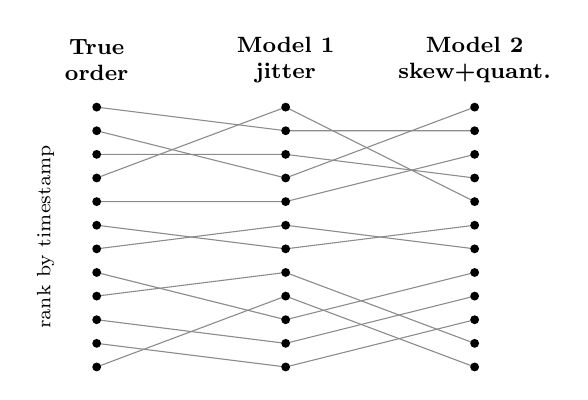
\begin{tikzpicture}[font=\footnotesize]
\draw[black!45, thin] (0,0.30) -- (2.4,1.20) -- (4.8,0.30);
\draw[black!45, thin] (0,0.60) -- (2.4,0.30) -- (4.8,0.90);
\draw[black!45, thin] (0,0.90) -- (2.4,0.60) -- (4.8,1.20);
\draw[black!45, thin] (0,1.20) -- (2.4,1.50) -- (4.8,0.60);
\draw[black!45, thin] (0,1.50) -- (2.4,0.90) -- (4.8,1.50);
\draw[black!45, thin] (0,1.80) -- (2.4,2.10) -- (4.8,1.80);
\draw[black!45, thin] (0,2.10) -- (2.4,1.80) -- (4.8,2.10);
\draw[black!45, thin] (0,2.40) -- (2.4,2.40) -- (4.8,3.00);
\draw[black!45, thin] (0,2.70) -- (2.4,3.60) -- (4.8,2.40);
\draw[black!45, thin] (0,3.00) -- (2.4,3.00) -- (4.8,2.70);
\draw[black!45, thin] (0,3.30) -- (2.4,2.70) -- (4.8,3.60);
\draw[black!45, thin] (0,3.60) -- (2.4,3.30) -- (4.8,3.30);
\fill (0,0.30) circle (1.6pt);
\fill (0,0.60) circle (1.6pt);
\fill (0,0.90) circle (1.6pt);
\fill (0,1.20) circle (1.6pt);
\fill (0,1.50) circle (1.6pt);
\fill (0,1.80) circle (1.6pt);
\fill (0,2.10) circle (1.6pt);
\fill (0,2.40) circle (1.6pt);
\fill (0,2.70) circle (1.6pt);
\fill (0,3.00) circle (1.6pt);
\fill (0,3.30) circle (1.6pt);
\fill (0,3.60) circle (1.6pt);
\fill (2.4,1.20) circle (1.6pt);
\fill (2.4,0.30) circle (1.6pt);
\fill (2.4,0.60) circle (1.6pt);
\fill (2.4,1.50) circle (1.6pt);
\fill (2.4,0.90) circle (1.6pt);
\fill (2.4,2.10) circle (1.6pt);
\fill (2.4,1.80) circle (1.6pt);
\fill (2.4,2.40) circle (1.6pt);
\fill (2.4,3.60) circle (1.6pt);
\fill (2.4,3.00) circle (1.6pt);
\fill (2.4,2.70) circle (1.6pt);
\fill (2.4,3.30) circle (1.6pt);
\fill (4.8,0.30) circle (1.6pt);
\fill (4.8,0.90) circle (1.6pt);
\fill (4.8,1.20) circle (1.6pt);
\fill (4.8,0.60) circle (1.6pt);
\fill (4.8,1.50) circle (1.6pt);
\fill (4.8,1.80) circle (1.6pt);
\fill (4.8,2.10) circle (1.6pt);
\fill (4.8,3.00) circle (1.6pt);
\fill (4.8,2.40) circle (1.6pt);
\fill (4.8,2.70) circle (1.6pt);
\fill (4.8,3.60) circle (1.6pt);
\fill (4.8,3.30) circle (1.6pt);
\node[font=\footnotesize\bfseries, align=center] at (0,4.2) {True\\order};
\node[font=\footnotesize\bfseries, align=center] at (2.4,4.2) {Model 1\\jitter};
\node[font=\footnotesize\bfseries, align=center] at (4.8,4.2) {Model 2\\skew+quant.};
\node[font=\scriptsize, rotate=90] at (-0.65,1.95) {rank by timestamp};
\end{tikzpicture}
\end{document}
